\section*{Đề thi thử THPTQG Sở GD\&ĐT HẢI PHÒNG 25--26, Lần 2}

\caulc
\Opensolutionfile{ans}[ans/ans-26-2-HAIPHONG-SoGD-L2-LC]
\begin{ex} %[1H4N4-2]
	Cho hình hộp $ABCD.A'B'C'D'$. Mệnh đề nào dưới đây là \textbf{sai}?
	\choice
	{$(BDA')\parallel(B'D'C) $}
	{\True $(ABA')\parallel(B'D'C) $}
	{$(ADD'A')\parallel (BCC'B') $}
	{$(ABCD)\parallel (A'B'C'D') $}
	\loigiai{
		\begin{center}
			\begin{tikzpicture}
				\def\a{3}
				\def\b{2}
				\def\h{3.5}
				\path 	(0:0) coordinate (A)
				++(0:\a) coordinate (D)
				++(-130:\b) coordinate (C)
				($(A)+(C)-(D)$) coordinate (B)
				($(A)+(75:\h)$) coordinate (A')
				($(B)+(75:\h)$) coordinate (B')
				($(C)+(75:\h)$) coordinate (C')
				($(D)+(75:\h)$) coordinate (D');
				\draw[dashed] 	(B)--(A)--(D)	(A)--(A')--(B);
				\draw	(C)--(C') 	(D)--(D') 	(B)--(B')	(C)--(C')
				(B)--(C)--(D) (B')--(D')--(C)--cycle
				(A')--(B')--(C')--(D')--cycle;
				\foreach \x/\g in {A/180,B/180,C/0,D/0,A'/180,B'/180,C'/0,D'/0}
				\fill[black] 	(\x) circle (1pt)
				($(\g:4mm)+(\x)$) node {$\x$};	
			\end{tikzpicture}
		\end{center}
		Ta có $\heva{&(ABA')\equiv (ABB'A')\\&B'\in d=(ABB'A')\cap (B'D'C)}\Rightarrow d=(ABA')\cap (B'D'C)$.\\
		Vậy hai mặt phẳng $(ABA')$ và $(B'D'C)$ không song song với nhau.
	}
\end{ex}
%============TN-02==============%
\begin{ex} %[2H2N1-2]
	Cho hình lập phương $ABCD.A'B'C'D'$ có cạnh bằng $a$. Độ dài của vectơ $\overrightarrow{u}=\overrightarrow{A'C'}-\overrightarrow{A'A}$ bằng
	\begin{center}
		\begin{tikzpicture}
			\def\a{3.3}
			\path 	(0:0) coordinate (A)
			++(0:\a) coordinate (D)
			++(-130:\a/2) coordinate (C)
			($(A)+(C)-(D)$) coordinate (B)
			($(A)+(90:\a)$) coordinate (A')
			($(B)+(90:\a)$) coordinate (B')
			($(C)+(90:\a)$) coordinate (C')
			($(D)+(90:\a)$) coordinate (D');
			\draw[dashed] 	(B)--(A)--(D)	(A)--(A');
			\draw	(C)--(C') 	(D)--(D') 	(B)--(B') 	(B)--(C)--(D) (A')--(B')--(C')--(D')--cycle;
			\foreach \x/\g in {A/180,B/180,C/0,D/0,A'/180,B'/180,C'/0,D'/0}
			\fill[black] 	(\x) circle (1pt)
			($(\g:4mm)+(\x)$) node {$\x$};	
		\end{tikzpicture}
	\end{center}
	\choice
	{$a\sqrt{6}$}
	{$a\sqrt{2}$}
	{$\dfrac{a\sqrt{3}}{2}$}
	{\True $a\sqrt{3}$}
	\loigiai
	{
		\begin{center}
			\begin{tikzpicture}
				\def\a{3.3}
				\path 	(0:0) coordinate (A)
				++(0:\a) coordinate (D)
				++(-130:\a/2) coordinate (C)
				($(A)+(C)-(D)$) coordinate (B)
				($(A)+(90:\a)$) coordinate (A')
				($(B)+(90:\a)$) coordinate (B')
				($(C)+(90:\a)$) coordinate (C')
				($(D)+(90:\a)$) coordinate (D');
				\draw[dashed] 	(B)--(A)--(D)	(A)--(A') (A)--(C) (A')--(C);
				\draw	(C)--(C') 	(D)--(D') 	(B)--(B') 	(B)--(C)--(D) (A')--(B')--(C')--(D')--cycle (A')--(C');
				\foreach \x/\g in {A/180,B/180,C/0,D/0,A'/180,B'/180,C'/0,D'/0}
				\fill[black] 	(\x) circle (1pt)
				($(\g:4mm)+(\x)$) node {$\x$};	
			\end{tikzpicture}
		\end{center}
		Ta  có $\left|\overrightarrow{u}\right|=\left|\overrightarrow{A'C'}-\overrightarrow{A'A}\right|=\left|\overrightarrow{A'C}\right|=A'C$.\\
		Trong tam giác $ ACA'$ có $A'C=\sqrt{AA'^2+AC^2}=\sqrt{a^2+2a^2}=a\sqrt{3}$.\\
		Vậy $\left|\overrightarrow{u}\right|=a\sqrt{3}$.
	}
\end{ex}
%============TN-03==============%
\begin{ex}%[2H5H2-7]
	Trong không gian $Oxyz$, cho hai đường thẳng $d_1\colon \heva{&x=t\\ &y=1-2t\\&z=-3t}$, $d_2\colon \dfrac{x}{-4}=\dfrac{y-1}{1}=\dfrac{z+1}{5}$. Góc giữa hai đường thẳng $d_1$, $d_2$ bằng bao nhiêu độ?
	\choice
	{\True $30^{\circ}$}
	{$45^{\circ}$}
	{$60^{\circ}$}
	{$90^{\circ}$}
	\loigiai{$d_1$, $d_2$ lần lượt có các vectơ chỉ phương là $\overrightarrow{u}_1=\left(1;-2;-3\right)$, $\overrightarrow{u}_2=\left(-4;1;5\right)$.\\
		Ta có $\cos\left(d_1,d_2\right)=\dfrac{\left|\overrightarrow{u}_1\cdot\overrightarrow{u}_2\right|}{\left|\overrightarrow{u}_1\right|\cdot\left|\overrightarrow{u}_2\right|}=\dfrac{\left|1\cdot(-4)-2\cdot 1-3\cdot 5\right|}{\sqrt{1^2+(-2)^2+(-3)^2}\cdot \sqrt{(-4)^2+1^2+5^2}}=\dfrac{\sqrt{3}}{2}.$\\
		Vậy $\left(d_1,d_2\right)=30^\circ$.
	}
\end{ex}
%============TN-04==============%
\begin{ex} %[2D1N4-1]
	Cho hàm số $f(x)$ liên tục trên mỗi khoảng $\left(-\infty;-\dfrac{1}{2} \right)$ và $\left(-\dfrac{1}{2};+\infty \right)$ và có bảng biến thiên như hình vẽ 
	\begin{center}
		
\begin{tikzpicture}[scale=0.8]
			\tkzTabInit %lgt= độ rộng cột x,f(x);espcl= độ rộng của cột
			{$x$/1,$y'$/1,$y$/3}
			{$-\infty$,$-\tfrac{1}{2}$,$+\infty$}
			\tkzTabLine{,+,d,+,} %d là không xác định
			\tkzTabVar{-/$2$,+D-/$+\infty$/$-\infty$,+/$2$}
			%+D+/$2$/$0$: 2 trái trên, giữa không xác định,0 phải trên
			%+D-/$2$/$0$: 2 trái trên, giữa không xác định,0 phải dưới
			%+DH/$2$: 2 trái trên, giữa không xác định đến tiếp theo
		\end{tikzpicture}
	\end{center}
	Tiệm cận ngang của đồ thị hàm số là đường thẳng có phương trình
	\choice
	{$x=2$}
	{\True $y=2$}
	{$x=-\dfrac{1}{2}$}
	{$y=-\dfrac{1}{2}$}
	\loigiai{Dựa vào bảng biến thiên hàm số ta có $\heva{&\lim\limits_{x\to +\infty}y=2\\&\lim\limits_{x\to -\infty}y=2.}$\\
		Vậy đồ thị hàm số có đường tiệm cận ngang là $y=2$.}
\end{ex}
%============TN-05==============%
\begin{ex}%[1D6N4-3]
	Tập nghiệm của bất phương trình $\log_{\tfrac{1}{6}}(x-2) >-1$ là
	\choice
	{$\left(2;\dfrac{13}{6} \right) $}
	{$\left(\dfrac{13}{6};+\infty \right) $}
	{\True $(2;8) $}
	{$(8;+\infty) $}
	\loigiai{\begin{eqnarray*}
			&&\log_{\tfrac{1}{6}}\left(x-2\right)>-1\\
			&\Leftrightarrow& 0<x-2<\left(\dfrac{1}{6}\right)^{-1}\\
			&\Leftrightarrow&2<x< 8.
		\end{eqnarray*}
		Vậy tập nghiệm của bất phương trình đã cho là $S=\left(2;8\right)$.}
\end{ex}
%============TN-06==============%
\begin{ex} %[2D1H5-1]
	\immini{Hình vẽ bên là đồ thị hàm số nào?
		\choice
		{$y=x^3-2x^2+1$}
		{\True $y=x^3-2x+1$}
		{$y=-x^3+2x^2+1$}
		{$y=x^3+2x^2+1$}}{\begin{tikzpicture}[scale=0.75,>=stealth, line join=round, line cap=round, every node/.style={font=\normalsize}, declare function={f(\x)=(\x)^3-2*\x+1; xcd=-sqrt(2/3); ycd=f(xcd); xct=sqrt(2/3); yct=f(xct); xmin=-3.5; xmax=4.5; ymin=-3.5; ymax=4.8;}]
			\draw[-Stealth, line width=1pt] (xmin, 0) -- (xmax, 0) node[below] {$x$};
			\draw[-Stealth, line width=1pt] (0, ymin) -- (0, ymax) node[shift={(-6pt,-5pt)}] {$y$};
			\fill (0,0) circle (1pt) node[shift={(-135:10pt)}] {$O$};
			
			\foreach \i in {-3, -2, -1, 1, 2, 3, 4} {
				\draw[line width=0.6pt] (\i, 1.5pt) -- (\i, -1.5pt) node[below] {$\i$};
			}
			
			\foreach \i in {-3, -2, -1, 1, 2, 3, 4} {
				\draw[line width=0.6pt] (1.5pt, \i) -- (-1.5pt, \i) node[left] {$\i$};
			}
			
			\begin{scope}
				\clip (xmin, ymin) rectangle (xmax, ymax);
				\draw[line width=1pt, smooth, samples=300, domain=xmin:xmax] plot (\x, {f(\x)});
			\end{scope}
			
		\end{tikzpicture}
	}
	\loigiai{Giả sử $(C)\colon y=ax^3+bx^2+cx+d$.\\
		Ta có $y'=3ax^2+2bx+c$.\\
		Gọi $x_1$, $x_2$ là hai điểm cực trị của hàm số.\\
		Dựa vào đồ thị ta có $\heva{&a>0\\&x_1\cdot x_2=\dfrac{c}{3a}<0}\Leftrightarrow\heva{&a>0\\&c<0.}$\\
		Dựa vào các phương án ta có đồ thị hàm số đã cho là $y=x^3-2x+1$.}
\end{ex}
%============TN-07==============%
\begin{ex}%[2H5H1-3]
	Trong không gian với hệ tọa độ $Oxyz$, cho điểm $M(2;-3;1)$ và mặt phẳng $(P)\colon 2x-2y+z+3=0$. Mặt phẳng đi qua điểm $M$ và song song với mặt phẳng $(P)$ có phương trình là
	\choice
	{$-2x-2y+z-11=0$}
	{\True $2x-2y+z-11=0$}
	{$2x-2y-z-11=0$}
	{$2x-2y+z+1=0$}
	\loigiai{Gọi $(Q)$ là mặt phẳng song song với $(P)$ và đi qua $M\left(2;-3;1\right)$.\\
		Vì $(Q)\parallel (P)$ nên $(Q)$ có dạng $2x-2y+z+d=0$ ($d\neq 3$).\\
		Vì $(Q)$ đi qua $M$ nên $2\cdot 2-2\cdot (-3)+1+d=0\Leftrightarrow d=-11$.\\
		Vậy phương trình mặt phẳng $(Q)$ là $2x-2y+z-11=0$.}
\end{ex}
%============TN-08==============%
\begin{ex} %[1D6N2-1]
	Biết $a$, $b$ là các số thực dương, khác $1$ thỏa mãn $\log_a b=3$. Giá trị $\log_{a^2} \dfrac{a}{\sqrt{b}}$ bằng
	\choice
	{$\dfrac{3}{2}$}
	{$\dfrac{5}{2}$}
	{\True $-\dfrac{1}{4}$}
	{$\dfrac{5}{8}$}
	\loigiai{Ta có $\log_{a^2} \dfrac{a}{\sqrt{b}}=\log_{a^2} a-\log_{a^2} \sqrt{b}=\dfrac{1}{2}-\dfrac{1}{4}\cdot \log_a b=\dfrac{1}{2}-\dfrac{1}{4}\cdot 3=-\dfrac{1}{4}.$}
\end{ex}
%============TN-09==============%
\begin{ex} %[1D1N5-3]
	Nghiệm của phương trình $\cos x=\cos \dfrac{\pi}{4}$ là
	\choice
	{$x=\dfrac{\pi}{6}+k2\pi$, $k \in \mathbb{Z}$}
	{$x=\pm \dfrac{\pi}{3}+k2\pi$, $k \in \mathbb{Z}$}
	{$x=-\dfrac{\pi}{6}+k2\pi$, $k \in \mathbb{Z}$}
	{\True $x=\pm \dfrac{\pi}{4}+k2\pi$, $k \in \mathbb{Z}$}
	\loigiai{Ta có $\cos x=\cos \dfrac{\pi}{4}\Leftrightarrow x=\pm \dfrac{\pi}{4}+k2\pi$, $k \in \mathbb{Z}$}
\end{ex}
%============TN-10==============%
\begin{ex} %[1D2H3-2]
	Cho cấp số nhân $(u_n)$ có số hạng đầu $u_1=2$ và $u_6=486$. Công bội $q$ bằng
	\choice
	{$q=\dfrac{3}{2}$}
	{\True $q=3$}
	{$q=5$}
	{ $q=\dfrac{2}{3}$}
	\loigiai{Vì $(u_n)$ là cấp số nhân với công bội $q$ nên ta có $$u_6=u_1\cdot q^5\Leftrightarrow q^5=\dfrac{u_6}{u_1}\Leftrightarrow q^5=\dfrac{486}{2}\Leftrightarrow q^5=243\Leftrightarrow q=3.$$
		Vậy công bội của cấp số nhân đã cho là $q=3$.}
\end{ex}
%============TN-11==============%
\begin{ex} %[2D4N2-1]
	Cho hàm số $f(x)$ liên tục trên $\mathbb{R}$. Biết hàm số $F(x)$ là một nguyên hàm của hàm số $f(x)$ trên $\mathbb{R}$ và $F(2)=6$, $F(4)=12$. Tích phân $\displaystyle\int\limits_{2}^{4} f(x)\mathrm{\,d}x$ bằng
	\choice
	{$-2$}
	{\True $6$}
	{$2$}
	{$18$}
	\loigiai{
		Ta có $\displaystyle\int\limits_{2}^{4} f(x)\mathrm{\,d}x=F(4)-F(2)=12-6=6$.
	}
\end{ex}
%============TN-12==============%
\begin{ex} %[1D5H1-3]
	Cân nặng (kg) của $50$ quả mít trong đợt thu hoạch của một trang trại được thống kê trong bảng dưới đây:
	\begin{center}
		\begin{tabular}{|c|c|c|c|c|c|}
			\hline
			Cân nặng (kg)&$\left[4;6\right)$&$\left[6;8\right)$&$\left[8;10\right)$& $\left[10;12\right)$&$\left[12;14\right)$\\
			\hline
			Số quả mít& $6$& $12$& $19$& $9$& $4$\\
			\hline
		\end{tabular}
	\end{center}
	Khối lượng trung bình của $50$ quả mít trên bảng
	\choice
	{\True $8{,}72$ kg}
	{$8{,}82$ kg}
	{$8{,}52$ kg}
	{$9{,}12$ kg}
	\loigiai{
		Ta có bảng giá trị đại diện như sau:	\begin{center}
			\begin{tabular}{|c|c|c|c|c|c|}
				\hline
				Cân nặng (kg)&$\left[4;6\right)$&$\left[6;8\right)$&$\left[8;10\right)$& $\left[10;12\right)$&$\left[12;14\right)$\\
				\hline
				Giá trị đại diện & $5$& $7$ & $9$ & $11$& $13$\\
				\hline
				Số quả mít& $6$& $12$& $19$& $9$& $4$\\
				\hline
			\end{tabular}
		\end{center}
		Vậy khối lượng trung bình của $50$ quả mít trên bảng là $$\overline{x}=\dfrac{5\cdot 6+7\cdot 12+9\cdot 19+11\cdot 9+13\cdot 4}{50}=8{,}72~(\text{kg}).$$
	}
\end{ex}

\Closesolutionfile{ans}


\cauds
\Opensolutionfile{ans}[ans/ans-26-2-HAIPHONG-SoGD-L2-DS]

\begin{ex}%[2D1V3-6]
	Giả sử lợi nhuận biên (tính bằng triệu đồng) của một sản phẩm được mô hình hóa bằng công thức $P'(x)=-0{,}04x+10$. Ở đây $P(x)$ là lợi nhuận (tính bằng triệu đồng) khi bán được $x$ đơn vị sản phẩm. Biết rằng khi chưa bán được sản phẩm nào, lợi nhuận của doanh nghiệp bằng $0$ (đã hòa vốn chi phí cố định).
	\choiceTF
	{Lợi nhuận khi bán được $x$ đơn vị sản phẩm được tính bằng công thức $P(x)=-0{,}04x^2+10x$}
	{\True Lợi nhuận khi bán được $100$ sản phẩm đầu tiên là $800$ triệu đồng}
	{\True Sự thay đổi của lợi nhuận khi doanh số tăng từ $100$ lên $150$ đơn vị sản phẩm là $250$ triệu đồng}
	{\True Biết sự thay đổi của lợi nhuận khi doanh số tăng từ $100$ lên $a$ đơn vị sản phẩm ($a \in \mathbb{N}^*$) lớn hơn $112$ triệu đồng, khi đó giá trị nhỏ nhất của $a$ là $121$}
	\loigiai{
		\begin{itemchoice}
			\itemch Ta có $P(x) = \displaystyle \int P'(x) \mathrm{\,d}x = \int (-0{,}04x + 10) \mathrm{\,d}x = -0{,}02x^2 + 10x + C$.\\
			Vì khi chưa bán được sản phẩm nào lợi nhuận bằng $0$ nên $P(0) = 0 \Rightarrow C = 0$.\\
			Vậy $P(x) = -0{,}02x^2 + 10x$.
			\itemch Lợi nhuận khi bán $100$ sản phẩm đầu tiên là $P(100) = -0{,}02 \cdot 100^2 + 10 \cdot 100 = 800$ triệu đồng.\\ 
			\itemch Sự thay đổi lợi nhuận là $P(150) - P(100) = \left(-0{,}02 \cdot 150^2 + 10 \cdot 150\right) - 800 = 1050 - 800 = 250$ triệu đồng.
			\itemch Sự thay đổi lợi nhuận từ $100$ lên $a$ là $P(a) - P(100) > 112$.\\
			Suy ra $-0{,}02a^2 + 10a - 800 > 112 \Leftrightarrow -0{,}02a^2 + 10a - 912 > 0$.\\
			Giải bất phương trình ta được $120 < a < 380$.\\
			Vì $a \in \mathbb{N}^*$ và cần tìm giá trị nhỏ nhất nên $a = 121$.
		\end{itemchoice}
	}
\end{ex}

\begin{ex}%[1H8V6-2]
	Cho lăng trụ đứng $ABC.A'B'C'$ có $AC=a$, $BC=2a$, $\widehat{ACB}=120^\circ$. Biết số đo góc nhị diện $[C', AB, C]$ bằng $60^\circ$.
	\choiceTF
	{\True Diện tích tam giác $ABC$ là $\dfrac{a^2\sqrt{3}}{2}$}
	{$CC'=\dfrac{a\sqrt{21}}{7}$}
	{\True Khoảng cách từ điểm $C$ đến mặt phẳng $\left(ABC'\right)$ là $\dfrac{3a\sqrt{7}}{14}$}
	{\True Khoảng cách giữa hai đường thẳng $BC$ và $AC'$ là $\dfrac{3a\sqrt{19}}{19}$}
	\loigiai{
		\begin{center}
			\begin{tikzpicture}[declare function={r=4;gocC=-47;}]
				\path (0,0) coordinate (A)
				(0:r) coordinate (B)
				(gocC:0.45*r)  coordinate (C)
				%%---------------------------%%
				(-90:1.2*r) coordinate (A')
				($(A')+(C)-(A)$) coordinate (C')
				($(A')+(B)-(A)$) coordinate (B')
				%%---------------------------%%
				($(A)!0.47!(B)$) coordinate (H)
				($(C')!0.7!(H)$) coordinate (K)
				;
				%%---------------------------%%
				\path pic[draw=red,fill=cyan,angle radius=10pt]{angle= C--H--C'};
				\foreach \x/\y/\z in {C/H/A,C/K/H}{
					\path pic[draw=red,angle radius=5pt]{right angle= \x--\y--\z};
				}
				%%---------------------------%%
				\draw (A)--(B)--(C)--(A)--(C')--(B)--(B')--(C')--(A')--cycle
				(C)--(C')		(C)--(H)
				;
				%%---------------------------%%
				\draw[dashed] (A')--(B')	(H)--(C')		(C)--(K);
				%%---------------------------%%
				\foreach \t/\g in {A/180,B/0,C/210,A'/180,B'/0,C'/-90,H/90,K/-10}{
					\fill[ball color=red] (\t) circle (1pt) node[shift={(\g:7pt)},font=\footnotesize]{$ \t $};
				}
			\end{tikzpicture}
		\end{center}
		\begin{itemchoice}
			\itemch Diện tích tam giác $ABC$ là $S_{ABC} = \dfrac{1}{2} AC \cdot BC \cdot \sin \widehat{ACB} = \dfrac{1}{2} \cdot a \cdot 2a \cdot \sin 120^\circ = \dfrac{a^2\sqrt{3}}{2}$.
			\itemch Áp dụng định lý hàm số cosin trong $\triangle ABC$
			\begin{eqnarray*}
				AB^2 &=& AC^2 + BC^2 - 2AC \cdot BC \cdot \cos 120^\circ \\
				&=& a^2 + 4a^2 - 2 \cdot a \cdot 2a \cdot \left(-\dfrac{1}{2}\right)\\ 
				&=& 7a^2.
			\end{eqnarray*}
			Suy ra $AB= a\sqrt{7}$.\\
			Kẻ $CH \perp AB$ tại $H$. Ta có $CH = \dfrac{2S_{ABC}}{AB} = \dfrac{a^2\sqrt{3}}{a\sqrt{7}} = \dfrac{a\sqrt{21}}{7}$.\\
			Vì $CC' \perp (ABC) \Rightarrow CC' \perp AB$. Mà $CH \perp AB \Rightarrow AB \perp \left(C'CH\right) \Rightarrow AB \perp C'H$.\\
			Vậy góc nhị diện $[C', AB, C]$ chính là góc $\widehat{C'HC} = 60^\circ$.\\
			Trong $\triangle C'CH$ vuông tại $C$ có 
			$CC' = CH \cdot \tan 60^\circ = \dfrac{a\sqrt{21}}{7} \cdot \sqrt{3} = \dfrac{a\sqrt{63}}{7} = \dfrac{3a\sqrt{7}}{7}$.
			\itemch Kẻ $CK \perp C'H$ tại $K$.\\		
			Vì $AB \perp \left(C'CH\right) \Rightarrow AB \perp CK$. Suy ra $CK \perp \left( ABC'\right)$.\\
			Khoảng cách từ $C$ đến $(ABC')$ là đường cao $CK$ của $\triangle C'CH$\\ 
			$\mathrm{d}(C, (ABC')) = CK = \dfrac{CC' \cdot CH}{\sqrt{CC'^2 + CH^2}}=\dfrac{\dfrac{a\sqrt{63}}{7}\cdot \dfrac{a\sqrt{21}}{7}}{\sqrt{\left(\dfrac{a\sqrt{63}}{7} \right)^2 + \left(\dfrac{a\sqrt{21}}{7} \right)^2}}=\dfrac{3a\sqrt{7}}{14}$.
			\itemch 
				Kẻ $AE \perp BC$ tại $E$, kẻ $A'D \perp B'C'$ tại $D$, kẻ $EF \perp AD$ tại $F$.
			\begin{center}
				\begin{tikzpicture}[declare function={r=4;gocC=-27;}]
					\path (0,0) coordinate (A)
					(0:r) coordinate (B)
					(gocC:0.65*r)  coordinate (C)
					%%---------------------------%%
					(-90:1.3*r) coordinate (A')
					($(A')+(C)-(A)$) coordinate (C')
					($(A')+(B)-(A)$) coordinate (B')
					%%---------------------------%%
					($(A)!0.37!(B)$) coordinate (H)
					($(C')!0.7!(H)$) coordinate (K)
					%%---------------------------%%
					($(C)!-0.45!(B)$) coordinate (E)
					($(E)+(C')-(C)$) coordinate (D)
					($(A)!0.30!(D)$) coordinate (F)
					;
					%%---------------------------%%
					%		\path pic[draw=red,fill=cyan,angle radius=10pt]{angle= C'--H--C};
					\foreach \x/\y/\z in {A/E/C,E/F/D}{
						\path pic[draw=red,angle radius=5pt]{right angle= \x--\y--\z};
					}
					%%---------------------------%%
					\path pic["\scriptsize$120^\circ$", angle eccentricity=1.7,draw,angle radius=7pt]{angle= B--C--A};
					%%---------------------------%%
					\draw (A)--(B)--(C)--(A) node [above,sloped,pos=0.5]{$a$}   
					(C')--(B)--(B')--(C')  (A')--(A)
					(C)--(C')		%(C)--(H)	
					(A)--(E)--(D)--(A')		(E)--(C)		(D)--(C')
					(A)--(D)		(E)--(F)
					;
					%%---------------------------%%
					\draw[dashed] (A')--(B')	(A)--(B') 		%(H)--(C')		(C)--(K)
					(A)--(C')		(A')--(C')		
					;
					%%---------------------------%%
					\foreach \t/\g in {A/180,B/0,C/-10,A'/180,B'/0,C'/-90,E/-20,D/-90,F/-130}{
						\fill[ball color=red] (\t) circle (1pt) node[shift={(\g:7pt)},font=\footnotesize]{$ \t $};
					}
				\end{tikzpicture}
			\end{center}
		
			Vì $\widehat{ACB}=120^\circ \Rightarrow \widehat{ACE}=60^\circ$.\\
			Trong $\triangle ACE$ vuông tại $E$ có $\sin\widehat{ACE}=\dfrac{AE}{AC}\Rightarrow AE = \dfrac{a\sqrt{3}}{2}$.\\
			Ta có $AE \perp BE$, $BE \perp DE$ suy ra $BE \perp \left(AED\right) \Rightarrow BE \perp EF$.\\
			Mà $EF \perp AD$ suy ra $EF \perp \left(AB'D \right)$. Hay $EF$ là khoảng cách từ $E$ đến $\left(AB'D\right)$.\\
			Lại có $BC \parallel B'D$ nên khoảng cách giữa hai đường thẳng $BC$ và $AC'$ bằng khoảng cách từ đường thẳng $BC$ đến $\left(AB'D \right)$ và bằng khoảng cách từ $E$ đến $\left(AB'D \right)$ bằng đoạn $EF$.\\
			Trong $\triangle ADE$ vuông tại $E$ có đường cao $EF$ suy ra $\dfrac{1}{EF^2}=\dfrac{1}{AE^2}+\dfrac{1}{DE^2}$.\\
			Suy ra 
			\begin{eqnarray*}
				EF&=&\dfrac{AE\cdot DE}{\sqrt{AE^2+DE^2}}\\
				&=&\dfrac{\dfrac{a\sqrt{3}}{2}\cdot \dfrac{a\sqrt{63}}{7}}{\sqrt{\left(\dfrac{a\sqrt{3}}{2}\right)^2+\left(\dfrac{a\sqrt{63}}{7}\right)^2}}\\
				&=& \dfrac{3a\sqrt{19}}{19}.
			\end{eqnarray*}
			Vậy khoảng cách giữa hai đường thẳng $BC$ và $AC'$ là $\dfrac{3a\sqrt{19}}{19}$.
			
		\textbf{	Cách khác:}
		\begin{center}
			\begin{tikzpicture}[declare function={r=4; gocC=-45; h=5.5;}, line join=round, line cap=round, >=stealth, font=\footnotesize]
				% 1. Định nghĩa tọa độ các đỉnh đáy dưới A'B'C'
				\coordinate (A') at (0,0);
				\coordinate (B') at (0:r);
				\coordinate (C') at (gocC:0.5*r);
				
				% 2. Định nghĩa tọa độ các đỉnh đáy trên ABC
				\coordinate (A) at ($(A')+(0,h)$);
				\coordinate (B) at ($(B')+(0,h)$);
				\coordinate (C) at ($(C')+(0,h)$);
				
				% 3. Các điểm phụ phục vụ tính khoảng cách d(A', (AB'C'))
				% I là hình chiếu của A' lên B'C'
				\coordinate (I) at ($(B')!(A')!(C')$); 
				% G là hình chiếu của A' lên AI
				\coordinate (G) at ($(A)!(A')!(I)$);
				
				% 4. Vẽ các mặt và cạnh thấy (Nét liền)
				\draw (A)--(B)--(C)--cycle; % Đáy trên
				\draw (A)--(A') (B)--(B') (C)--(C'); % Các cạnh bên
				\draw (A')--(C')--(B'); % Các cạnh thấy đáy dưới
				\draw  (A)--(C'); % Các cạnh thấy của mặt phẳng (AB'C')
				
				% 5. Vẽ các cạnh khuất (Nét đứt)
				\draw[dashed, thick] (A')--(B') (A)--(B') (A)--(I); % Cạnh khuất đáy dưới
				\draw (A')--(I) --(C'); % Đoạn cao đáy và giao tuyến AI
				\draw[dashed, thick] (A')--(G); % Đoạn khoảng cách cần tìm
				
				% 6. Ký hiệu các góc vuông
				\path pic[draw, thin, angle radius=6pt]{right angle= A'--I--B'};
				\path pic[draw, thin, angle radius=6pt]{right angle= A'--G--A};
				\path pic[draw, thin, angle radius=6pt]{right angle= A--A'--I};
				
				% 7. Vẽ các điểm và hiển thị nhãn (Đã fix lỗi góc số bằng định hướng chữ)
				\foreach \t/\g in {A/above left, B/above right, C/right, A'/left, B'/right, C'/below, I/below, G/above left}{
					\fill (\t) circle (1.5pt);
					\node[\g] at (\t) {$\t$};
				}
			\end{tikzpicture}
		\end{center}
		
		Do $BC \parallel B'C'$ nên đường thẳng $BC \parallel (AB'C')$. \\
		Mà $AC' \subset (AB'C')$, do đó khoảng cách giữa hai đường thẳng chéo nhau $BC$ và $AC'$ được quy về khoảng cách từ một điểm trên $BC$ đến mặt phẳng $(AB'C')$:
		$$\mathrm{d}(BC, AC') = \mathrm{d}(BC, (AB'C')) = \mathrm{d}(B, (AB'C')).$$
		Mặt khác, đoạn thẳng $BB'$ cắt mặt phẳng $(AB'C')$ tại trung điểm $B'$ của nó (hoặc xét tính đối xứng qua các mặt bên), ta dễ dàng có được mối liên hệ khoảng cách từ hai đỉnh đối diện đáy đến mặt phẳng này là bằng nhau:
		$$\mathrm{d}(B, (AB'C')) = \mathrm{d}(A', (AB'C')).$$
		Hình chiếu vuông góc của đỉnh $A'$ lên mặt phẳng $(AB'C')$ chính là đường cao kẻ từ đỉnh góc vuông của tứ diện vuông cụ thể hoặc lăng trụ. Ta hạ $A'I \perp B'C'$ tại $I$. \\
		Vì lăng trụ đứng nên $AA' \perp (A'B'C') \Rightarrow AA' \perp B'C'$. Từ đó $B'C' \perp (AA'I) \Rightarrow (AB'C') \perp (AA'I)$. \\
		Trong mặt phẳng $(AA'I)$, kẻ $A'G \perp AI$ tại $G$. Khi đó $A'G \perp (AB'C')$, tức là $\mathrm{d}(A', (AB'C')) = A'G$.
		
		Tính toán các giá trị trong tam giác đáy $A'B'C'$ (đối xứng hoàn toàn với $\triangle ABC$):
		\begin{itemize}
			\item Diện tích đáy: $S_{\triangle A'B'C'} = S_{\triangle ABC} = \dfrac{a^2\sqrt{3}}{2}$.
			\item Cạnh $B'C' = BC = 2a$.
			\item Đường cao đáy $A'I$: $A'I = \dfrac{2S_{\triangle A'B'C'}}{B'C'} = \dfrac{a^2\sqrt{3}}{2a} = \dfrac{a\sqrt{3}}{2}$.
		\end{itemize}
		Xét tam giác $AA'I$ vuông tại $A'$ có đường cao $A'G$, với $AA' = CC' = \dfrac{3a\sqrt{7}}{7}$, ta có:
		$$\mathrm{d}(BC, AC') = A'G = \dfrac{AA' \cdot A'I}{\sqrt{AA'^2 + A'I^2}} = \dfrac{\dfrac{3a\sqrt{7}}{7} \cdot \dfrac{a\sqrt{3}}{2}}{\sqrt{\left(\dfrac{3a\sqrt{7}}{7}\right)^2 + \left(\dfrac{a\sqrt{3}}{2}\right)^2}} = \dfrac{3a\sqrt{19}}{19}.$$
		Vậy khoảng cách giữa hai đường thẳng $BC$ và $AC'$ là $\dfrac{3a\sqrt{19}}{19}$.
		
		\end{itemchoice}
	}
\end{ex}

\begin{ex}%[2D5V1-4]
	Một chiến dịch xét nghiệm tầm soát diện rộng được tổ chức để phát hiện sớm một căn bệnh truyền nhiễm. Theo thống kê y tế, tỉ lệ người mắc bệnh này trong cộng đồng là $1\%$. Loại test nhanh được sử dụng có độ nhạy là $99\%$ (cho kết quả dương tính với $99\%$ người bệnh) và độ đặc hiệu là $96\%$ (cho kết quả âm tính với $96\%$ người không mắc bệnh).
	\choiceTF
	{\True Xác suất xét nghiệm cho cho kết quả âm tính của một người mắc bệnh là $0{,}01$}
	{\True Xác suất xét nghiệm cho kết quả dương tính của một người không mắc bệnh là $0{,}04$}
	{Xác suất để một người bất kỳ trong cộng đồng đi xét nghiệm nhận kết quả dương tính là $0{,}05$}
	{\True Biết rằng một người có kết quả test nhanh là dương tính, xác suất để người đó thực sự mắc bệnh là $20\%$}
	\loigiai{
		Gọi $B$ là biến cố \lq\lq Người đi xét nghiệm mắc bệnh\rq\rq 
		$\Rightarrow \mathrm{P}(B) = 1\% = 0{,}01$ và $\mathrm{P}(\overline{B}) = 0{,}99$.\\
		Gọi $A$ là biến cố \lq\lq Kết quả xét nghiệm dương tính\rq\rq. Theo đề bài
		\begin{itemize}
			\item Độ nhạy: $\mathrm{P}(A|B) = 99\% = 0{,}99$.
			\item Độ đặc hiệu: $\mathrm{P}(\overline{A}|\overline{B}) = 96\% = 0{,}96$.
		\end{itemize}
	\begin{center}
		\begin{tikzpicture}[
			grow=right, 
			level 1/.style={sibling distance=3.5cm, level distance=4.5cm},
			level 2/.style={sibling distance=1.8cm, level distance=4.5cm},
			edge from parent/.style={draw, ->, >=stealth, thick},
			every node/.style={font=\footnotesize},
			sloped
			]
			
			\node {Cộng đồng}
			child {
				node[draw, rectangle] {$\overline{B}$ (Không bệnh)}
				child {
					node[draw, rectangle] {$\overline{A}$ (Âm tính)}
					edge from parent node[below] {$0{,}96$}
				}
				child {
					node[draw, rectangle] {$A$ (Dương tính)}
					edge from parent node[above] {$0{,}04$}
				}
				edge from parent node[below] {$\mathrm{P}(\overline{B}) = 0{,}99$}
			}
			child {
				node[draw, rectangle] {$B$ (Mắc bệnh)}
				child {
					node[draw, rectangle] {$\overline{A}$ (Âm tính)}
					edge from parent node[below] {$0{,}01$}
				}
				child {
					node[draw, rectangle] {$A$ (Dương tính)}
					edge from parent node[above] {$0{,}99$}
				}
				edge from parent node[above] {$\mathrm{P}(B) = 0{,}01$}
			};
		\end{tikzpicture}
	\end{center}
		\begin{itemchoice}
			\itemch Xác suất âm tính giả (mắc bệnh nhưng âm tính) là $\mathrm{P}(\overline{A}|B) = 1 - \mathrm{P}(A|B) = 1 - 0{,}99 = 0{,}01$.
			\itemch Xác suất dương tính giả (không mắc bệnh nhưng dương tính) là 
			$$\mathrm{P}(A|\overline{B}) = 1 - \mathrm{P}(\overline{A}|\overline{B}) = 1 - 0{,}96 = 0{,}04.$$
			\itemch Xác suất dương tính trong cộng đồng là
			$$\mathrm{P}(A) = \mathrm{P}(B) \cdot \mathrm{P}(A|B) + \mathrm{P}(\overline{B}) \cdot \mathrm{P}(A|\overline{B}) = 0{,}01 \cdot 0{,}99 + 0{,}99 \cdot 0{,}04 = 0{,}0099 + 0{,}0396 = 0{,}0495.$$
			\itemch Xác suất người đó thực sự mắc bệnh khi biết kết quả dương tính là
			$$\mathrm{P}(B|A) = \dfrac{\mathrm{P}(B \cap A)}{\mathrm{P}(A)} = \dfrac{0{,}0099}{0{,}0495} = \dfrac{1}{5} = 20\%.$$
		\end{itemchoice}
	}
\end{ex}
\begin{ex}%[2D1H3-1]
	Cho hàm số $y = f(x) = \ln(4ex - x^2)$.
	\choiceTF
	{ $f(2e) = 4$}
	{ Hàm số có tập xác định là $[0; 4e]$}
	{\True Phương trình $f'(x) = 0$ có một nghiệm $x = 2e$}
	{\True Giá trị lớn nhất của hàm số đã cho trên đoạn $[e; 3e]$ có dạng $a\ln 2 + b$ thì $a + b = 4$}
	\loigiai
	{
		\begin{itemchoice}
			\itemch Thay $x = 2e$ vào hàm số ta được $f(2e) = \ln(4e\cdot 2e - (2e)^2) = \ln(4e^2) = \ln 4 + \ln(e^2) = 2\ln 2 + 2 \neq 4$.
			\itemch Điều kiện xác định là $4e\cdot x - x^2 > 0 \Leftrightarrow x(4e - x) > 0 \Leftrightarrow 0 < x < 4e$. \\ 
			Vậy tập xác định của hàm số là $(0; 4e)$.
			\itemch Ta có $f'(x) = \dfrac{(4e\cdot x - x^2)'}{4e\cdot x - x^2} = \dfrac{4e - 2x}{4e\cdot x - x^2}$.\\
			Phương trình $f'(x) = 0 \Leftrightarrow 4e - 2x = 0 \Leftrightarrow x = 2e$ (thỏa mãn điều kiện $0 < x < 4e$).
			\itemch Trên đoạn $[e; 3e]$, ta có $f'(x) = 0 \Leftrightarrow x = 2e$.\\
			Tính các giá trị tại các điểm đầu mút và điểm cực trị:\\
			$f(e) = \ln(4e\cdot e - e^2) = \ln(3e^2) = \ln 3 + 2$.\\
			$f(3e) = \ln(4e\cdot 3e - (3e)^2) = \ln(3e^2) = \ln 3 + 2$.\\
			$f(2e) = \ln(4e\cdot 2e - (2e)^2) = \ln(4e^2) = 2\ln 2 + 2$.\\
			So sánh các giá trị ta thấy giá trị lớn nhất của hàm số trên đoạn $[e; 3e]$ là $2\ln 2 + 2$.\\
			Theo đề bài, giá trị lớn nhất có dạng $a\ln 2 + b$, suy ra $a = 2$ và $b = 2$.\\
			Khi đó $a + b = 2 + 2 = 4$.
		\end{itemchoice}
	}
\end{ex}
\Closesolutionfile{ans}

\caukq
\Opensolutionfile{ans}[ans/ans-26-2-HAIPHONG-SoGD-L2-KQ]
\begin{ex}%[2D1V3-6]
	Để hỗ trợ học sinh ôn thi tốt nghiệp THPT, một nhóm chuyên gia đã phát triển ứng dụng trợ lý học tập $AI$. Số lượng người dùng ứng dụng sau $t$ tháng phát hành được mô hình hóa bởi hàm số:
	$$f(t) = \dfrac{12000}{1 + 23e^{-0,5t}}$$
	(Trong đó, thời gian $t \ge 0$ tính bằng tháng). Biết rằng hàm số $f'(t)$ biểu thị tốc độ tăng trưởng người dùng mới của ứng dụng. Sau khi phát hành bao nhiêu tháng thì tốc độ tăng trưởng người dùng của ứng dụng đạt giá trị lớn nhất? (Kết quả làm tròn đến hàng đơn vị).
	
	\shortans[oly]{$6$}
	\loigiai{
		Tốc độ tăng trưởng người dùng mới của ứng dụng được biểu thị bởi hàm số $f'(t)$.\\
		Ta có
		$$f'(t) = \dfrac{12000 \cdot 11{,5}e^{-0{,}5t}}{\left(1 + 23e^{-0{,}5t}\right)^2} = \dfrac{138000e^{-0{,}5t}}{\left(1 + 23e^{-0{,}5t}\right)^2}$$		
		Đặt $u = e^{-{0,5}t}$ với $0 < u \le 1$ do $t \ge 0$. Xét hàm số $g(u) = \dfrac{138000u}{(1 + 23u)^2}$ trên khoảng $(0; 1]$.\\		
		Áp dụng bất đẳng thức Cô-si cho hai số dương $1$ và $23u$, ta có
		$$(1 + 23u)^2 \ge \left(2\sqrt{23u}\right)^2 = 92u$$
		Do đó
		$$g(u) \le \dfrac{138000u}{92u} = 1500$$		
		Dấu \lq\lq=\rq\rq xảy ra khi và chỉ khi
		$1 = 23u \Leftrightarrow u = \dfrac{1}{23}$.\\		
		Thay ngược lại biến $t$, ta được
		$$e^{-0{,}5t} = \dfrac{1}{23} \Leftrightarrow -0{,}5t = \ln\left(\dfrac{1}{23}\right) \Leftrightarrow t = 2\ln 23 \approx 6\text{ (tháng)}.$$		
	}
\end{ex}

\begin{ex}%[0D2C2-3]
	Một xưởng gia công cơ khí chính xác nhận hợp đồng sản xuất hai loại linh kiện là Trục thép (Loại $A$) và Bánh răng (Loại $B$). Để sản xuất một lô linh kiện loại $A$ cần chạy máy Phay CNC trong $2$ giờ và máy Tiện CNC trong $4$ giờ. Để sản xuất một lô linh kiện loại $B$ cần chạy máy Phay CNC trong $3$ giờ và máy Tiện CNC trong $2$ giờ. Do yêu cầu bảo trì, mỗi tuần máy Phay CNC chỉ hoạt động tối đa $120$ giờ và máy Tiện CNC hoạt động tối đa $160$ giờ. Biết mỗi lô linh kiện loại $A$ cho lợi nhuận $3$ triệu đồng, mỗi lô linh kiện loại $B$ cho lợi nhuận $4$ triệu đồng và xưởng luôn tiêu thụ hết số sản phẩm làm ra. Hỏi mỗi tuần xưởng cơ khí thu được lợi nhuận cao nhất là bao nhiêu triệu đồng?
	
	\shortans[oly]{$170$}
	\loigiai{
		Gọi $x$, $y$ lần lượt là số lô linh kiện loại $A$ và loại $B$ mà xưởng sản xuất trong một tuần ($x, y$ là số tự nhiên).\\		
		Từ điều kiện giới hạn thời gian hoạt động của các loại máy trong tuần, ta có hệ bất phương trình ràng buộc sau
		$$\heva{& x \ge 0 \\& y \ge 0 \\& 2x + 3y \le 120 \\& 4x + 2y \le 160} \Leftrightarrow \heva{& x \ge 0 \\& y \ge 0 \\& 2x + 3y \le 120 \\& 2x + y \le 80.}$$		
		Tổng lợi nhuận mỗi tuần của xưởng (đơn vị: triệu đồng) được biểu thị qua hàm số số bậc nhất hai ẩn
		$F(x; y) = 3x + 4y$.\\
		Miền nghiệm của hệ bất phương trình trên là miền tứ giác $OABC$ (bao gồm cả các cạnh) trên mặt phẳng tọa độ $Oxy$, với tọa độ các đỉnh là
		$O(0; 0)$, $A(40; 0)$, $C(0; 40)$.\\
		Tọa độ đỉnh $B$ là nghiệm của hệ phương trình
		$$\heva{& 2x + 3y = 120 \\& 2x + y = 80} \Leftrightarrow \heva{& x = 30 \\& y = 20} \Rightarrow B(30; 20)$$
		\begin{center}
			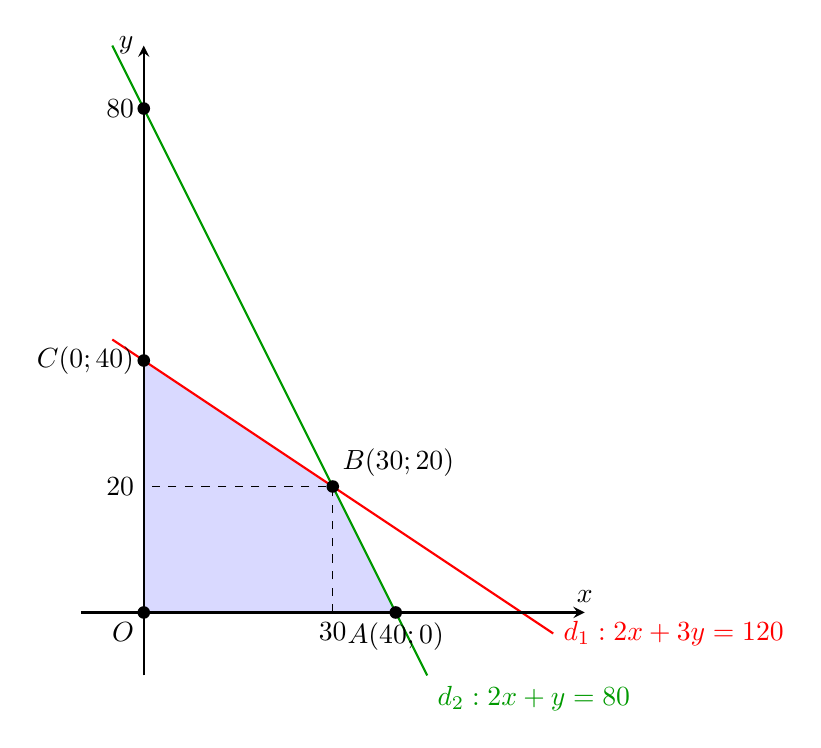
\begin{tikzpicture}[scale=0.08, >=stealth]
				% Tô màu miền nghiệm OABC
				\fill[color=blue!15] (0,0) -- (40,0) -- (30,20) -- (0,40) -- cycle;
				
				% Vẽ các đường thẳng
				% d1: 2x + 3y = 120  => y = (120 - 2x)/3
				% Cho x=0 => y=40; x=60 => y=0
				\draw[thick, color=red, domain=-5:65] plot (\x, {(120 - 2*\x)/3}) node[right] {$d_1: 2x + 3y = 120$};
				
				% d2: 2x + y = 80 => y = 80 - 2x
				% Cho x=0 => y=80; x=40 => y=0
				\draw[thick, color=green!60!black, domain=-5:45] plot (\x, {80 - 2*\x}) node[below right] {$d_2: 2x + y = 80$};
				
				% Vẽ hệ trục tọa độ Oxy
				\draw[->, thick] (-10,0) -- (70,0) node[above] {$x$};
				\draw[->, thick] (0,-10) -- (0,90) node[left] {$y$};
				
				% Gán nhãn các đỉnh của miền nghiệm
				\node[below left] at (0,0) {$O$};
				\node[below] at (40,0) {$A(40;0)$};
				\node[above right] at (30,20) {$B(30;20)$};
				\node[left] at (0,40) {$C(0;40)$};
				
				% Vẽ các điểm chấm tròn tại các đỉnh
				\fill (0,0) circle (1);
				\fill (40,0) circle (1);
				\fill (30,20) circle (1);
				\fill (0,40) circle (1);
				
				% Vẽ đường nét đứt gióng tọa độ điểm B
				\draw[dashed] (30,0) -- (30,20) -- (0,20);
				\node[below] at (30,0) {$30$};
				\node[left] at (0,20) {$20$};
				
				% Gán thêm một vài giá trị đặc biệt trên trục để đồ thị cân đối
				\node[left] at (0,80) {$80$};
				\fill (0,80) circle (1);
			\end{tikzpicture}
		\end{center}
		Tính giá trị của hàm lợi nhuận $F(x; y)$ tại các đỉnh của miền đa giác nghiệm:
		\begin{itemize}
			\item $F(0; 0) = 3 \cdot 0 + 4 \cdot 0 = 0$
			\item $F(40; 0) = 3 \cdot 40 + 4 \cdot 0 = 120$
			\item $F(30; 20) = 3 \cdot 30 + 4 \cdot 20 = 170$
			\item $F(0; 40) = 3 \cdot 0 + 4 \cdot 40 = 160$
		\end{itemize}		
		So sánh các giá trị, ta thấy giá trị lớn nhất của hàm số là $\max F = 170$ tại $B(30; 20)$.\\		
		Vậy mỗi tuần xưởng cơ khí thu được lợi nhuận cao nhất là $170$ triệu đồng.
	}
\end{ex}

\begin{ex}%[2D4C3-5]
	\immini[thm]
	{Một xưởng thủy tinh mỹ nghệ cần sản xuất những chiếc bình thủy tinh cỡ lớn để ngâm một loại sâm. Chiếc bình được tạo hình bằng cách quay hình phẳng $(H)$ (phần gạch chéo trong hình vẽ) quanh trục $AB$. Hình $(H)$ nằm trong hình chữ nhật $ABCD$, giới hạn bởi các đoạn thẳng $AM, BP$ (với $M, P$ lần lượt thuộc các cạnh $AD, BC$, $MP \parallel AB$), cung tròn $MN$ (có tâm $I$ là trung điểm của đoạn thẳng $AE$ nằm trên trục $AB$) và cung parabol $NP$. Biết $AB = 5$ dm, $AM = 1{,}5$ dm, $BP = 1{,}5$ dm, $BE = 1$ dm. Tiếp tuyến của cung tròn và cung parabol tại điểm tiếp giáp $N$ là trùng nhau để đảm bảo thành bình mượt mà, chịu lực tốt và đảm bảo tính thẩm mỹ. Giả sử bề dày của thành thủy tinh không đáng kể. Hỏi chiếc bình ngâm sâm này có sức chứa tối đa khoảng bao nhiêu lít nước? (Kết quả làm tròn đến hàng phần chục).
	}
	{
		\begin{tikzpicture}[scale=1,>=stealth, font=\footnotesize, line join=round, line cap=round,rotate=90]
			\fill[pattern=north east lines,opacity=0.6] plot[domain=0:4](\x,{sqrt(5-(\x-2)^2)})--plot[domain=4:5](\x,{2*(\x)^2-18*(\x)+41})--(5,0)--(0,0)--cycle;
			\draw (0,0)node[below right]{$A$}--(0,2.5)node[below left]{$D$}--(5,2.5)node[above left]{$C$}--(5,0)node[above right]{$B$}--cycle;
			\draw[dashed] (0,1)node[below]{$M$}--(5,1)node[above]{$P$} (4,1)node[above left]{$N$}--(4,0)node[right]{$E$};
			\draw[smooth,samples=300,domain=0:4] plot(\x,{sqrt(5-(\x-2)^2)});
			\draw[smooth,samples=300,domain=4:5] plot(\x,{2*(\x)^2-18*(\x)+41});
		\end{tikzpicture}
	}
	\shortans[oly]{$66{,}9$}
	\loigiai{
		\begin{center}
			\begin{tikzpicture}[scale=1.6, >=stealth, font=\footnotesize, line join=round, line cap=round]
				\coordinate (A) at (0,0);
				\coordinate (B) at (5,0);
				\coordinate (C) at (5,2.5);
				\coordinate (D) at (0,2.5);
				\coordinate (M) at (0,1);
				\coordinate (P) at (5,1);
				\coordinate (N) at (4,1);
				\coordinate (E) at (4,0);
				\fill[pattern=north east lines,opacity=0.6]
				plot[domain=0:4] ({\x}, {sqrt(5-(\x-2)^2)})
				-- plot[domain=4:5] ({\x}, {2*(\x)^2 - 18*(\x) + 41})
				-- (5,0) -- (0,0) -- cycle;
				\draw (A) node[below left]{$O$}
				-- (D) node[above left]{$D$}
				-- (C) node[above right]{$C$}
				-- (B) node[below right]{$B$}
				-- cycle;
				\draw[dashed] (M) node[left]{$M$} -- (P) node[right]{$P$};
				\draw[dashed] (N) node[above right]{$N$} -- (E) node[below]{$E$};
				\draw[smooth,samples=200,domain=0:4] plot(\x,{sqrt(5-(\x-2)^2)});
				\draw[smooth,samples=200,domain=4:5] plot(\x,{2*(\x)^2 - 18*(\x) + 41});
				\draw[->] (A) -- ($(A)+(6,0)$) node[right]{$x$};
				\draw[->] (A) -- ($(A)+(0,3)$) node[above]{$y$};
				\node at (2,1.9) {$y = f(x)$};
				\node at (4.6,0.4) {$y = g(x)$};
				
			\end{tikzpicture}
		\end{center}
		Chọn hệ trục tọa độ $Oxy$ sao cho gốc tọa độ $O \equiv A(0;0)$, trục $Ox$ trùng với đường thẳng $AB$ (chiều dương từ $A$ đến $B$), trục $Oy$ trùng với đường thẳng $AD$.\\
		Theo giả thiết, ta có các tọa độ điểm: $B(5;0)$. Do $BE = 1\text{ dm} \Rightarrow AE = 4\text{ dm} \Rightarrow E(4;0)$.\\
		Tâm $I$ của cung tròn là trung điểm của $AE$ nên $I(2;0)$. Do điểm $M \in AD$ và $AM = 1{,}5$ dm nên $M(0;1{,}5)$.\\		
		Bán kính của cung tròn $MN$ là
		$$R = IM = \sqrt{(0-2)^2 + 1{,}5^2} = \sqrt{4 + 2{,}25} = \sqrt{6{,}25} = 2{,}5\text{ dm}.$$
		Phương trình đường tròn tâm $I(2;0)$ bán kính $R=2{,}5$ là
		$$(x-2)^2 + y^2 = 6{,}25 \Rightarrow y^2 = 6{,}25 - (x-2)^2.$$
		Do cung $MN$ nằm ở góc phần tư thứ nhất ($y > 0$) nên phương trình cung $MN$ là
		$$y = f_1(x) = \sqrt{6{,}25 - (x-2)^2}.$$
		Vì điểm $N$ có hoành độ bằng hoành độ điểm $E$ nên $x_N = 4 \Rightarrow y_N = \sqrt{6{,}25 - (4-2)^2} = 1{,}5$. Vậy $N(4;1{,}5)$.\\
		Thể tích khối tròn xoay tạo thành khi quay phần cung $MN$ quanh trục $Ox$ là
		$$V_1 = \pi \displaystyle\int\limits_{0}^{4} f_1^2(x) \mathrm{\,d}x = \pi \int_{0}^{4} \left[6{,}25 - (x-2)^2\right] \mathrm{\,d}x = \dfrac{59\pi}{3}\text{ (dm}^3\text{)}.$$
		
		Gọi $y = f_2(x) = ax^2 + bx + c$ là hàm số của cung parabol $NP$. Do parabol đi qua $N(4;1{,}5)$ và $P(5;1{,}5)$ nên nó nhận đường thẳng $x = 4{,}5$ làm trục đối xứng, từ đó ta có biểu diễn
		$$f_2(x) = a(x-4)(x-5) + 1{,}5.$$
		Đạo hàm của hàm số cung tròn tại điểm tiếp giáp $N(4;1{,}5)$ là
		$$f_1'(4) = \left. \dfrac{-(x-2)}{\sqrt{6{,}25 - (x-2)^2}} \right|_{x=4} = -\dfrac{4}{3}.$$
		Vì tiếp tuyến của cung tròn và cung parabol tại $N$ trùng nhau nên:
		$$f_2'(4) = f_1'(4) \Leftrightarrow a(4-5) + a(4-4) = -\dfrac{4}{3} \Leftrightarrow -a = -\dfrac{4}{3} \Leftrightarrow a = \dfrac{4}{3}.$$
		Suy ra hàm số cung parabol là
		$$f_2(x) = \dfrac{4}{3}(x-4)(x-5) + 1{,}5 = \dfrac{4}{3}x^2 - 12x + \dfrac{169}{6}.$$
		Thể tích khối tròn xoay tạo thành khi quay phần cung $NP$ quanh trục $Ox$ là
		$$V_2 = \pi \displaystyle\int\limits_{4}^{5} f_2^2(x) \mathrm{d}x = \pi \displaystyle\int\limits_{4}^{5} \left(\frac{4}{3}x^2 - 12x + \frac{169}{6}\right)^2 \mathrm{\,d}x = \frac{887\pi}{540}\text{ (dm}^3\text{)}.$$		
		Sức chứa tối đa của chiếc bình ngâm sâm là tổng thể tích của hai phần
		$$V = V_1 + V_2 = \frac{59\pi}{3} + \frac{887\pi}{540} = \frac{11507\pi}{540} \approx 66{,}9\text{ (dm}^3\text{)} = 66{,}9\text{ (lít)}.$$
	}
\end{ex}
\begin{ex}%[1H8V7-2]
	Cho hình chóp $S.ABC$ có đáy là tam giác vuông cân tại $B$, $AB = 2\text{ cm}$. Cạnh bên $SA$ vuông góc với mặt phẳng đáy, $SA = 2\sqrt{3}\text{ cm}$. Gọi điểm $H$ là hình chiếu của điểm $A$ trên cạnh $SB$. Khi đó thể tích khối chóp $B.AHC$ bằng bao nhiêu $\text{cm}^3$? (Kết quả làm tròn đến hàng phần trăm).
	\shortans[oly]{$0{,}58$}
	\loigiai{
		\begin{center}
			\begin{tikzpicture}[font=\footnotesize, line join=round, line cap=round, >=stealth, scale=1.3]
					\path (0,0) coordinate (A) (0,2) coordinate (S) (-40:1.5) coordinate (B) (3.5,0) coordinate (C) ;
					\coordinate (H) at ($(S)!2/5!(B)$);
					\draw (S)--(A)--(B)--(C)--cycle (S)--(B) (A)--(H)--(C);
					\draw[dashed] (A)--(C);
					\pic [draw, angle radius=0.25cm] {right angle = S--A--B};
					\pic [draw, angle radius=0.25cm] {right angle = S--A--C};
					\pic [draw, angle radius=0.2cm] {right angle = A--H--B};
					\pic [draw, angle radius=0.2cm] {right angle = A--B--C};
					\foreach \x/\g in {S/90, A/180, B/-90, C/0, H/45}{
						\fill (\x) circle (1pt)+(\g:0.3)node{$\x$};
					}
				\end{tikzpicture}
		\end{center}
		Diện tích đáy $\triangle ABC$ là
	$$ S_{\triangle ABC} = \dfrac{1}{2} \cdot AB \cdot BC = \dfrac{1}{2} \cdot 2 \cdot 2 = 2 \text{ (cm}^2\text{)} $$
		Thể tích khối chóp $S.ABC$ là
		\[ V_{S.ABC} = \dfrac{1}{3} \cdot SA \cdot S_{\triangle ABC} = \dfrac{1}{3} \cdot 2\sqrt{3} \cdot 2 = \dfrac{4\sqrt{3}}{3} \text{ (cm}^3\text{)} \]
		Ta xét tam giác $SAB$ vuông tại $A$, có đường cao $AH$. Độ dài cạnh huyền $SB$ là
		\[ SB = \sqrt{SA^2 + AB^2} = \sqrt{(2\sqrt{3})^2 + 2^2} = \sqrt{12 + 4} = 4 \text{ (cm)} \]
		Áp dụng hệ thức lượng trong tam giác vuông $SAB$, ta có
		\[ SA^2 = SH \cdot SB \Rightarrow SH = \dfrac{SA^2}{SB} = \dfrac{12}{4} = 3 \text{ (cm)} \]
		Suy ra $\dfrac{SH}{SB} = \dfrac{3}{4}$, do đó $\dfrac{BH}{SB} = \dfrac{1}{4}$.
		Khi đó
		\[ \dfrac{V_{C.ABH}}{V_{C.SAB}} = \dfrac{S_{\triangle ABH}}{S_{\triangle SAB}} = \dfrac{BH}{SB} = \dfrac{1}{4} \]
		Vậy thể tích khối chóp $B.AHC$ là
		\[ V_{B.AHC} = \dfrac{1}{4} \cdot V_{S.ABC} = \dfrac{1}{4} \cdot \dfrac{4\sqrt{3}}{3} = \dfrac{\sqrt{3}}{3} \approx 0{,}58 \text{ (cm}^3\text{)} \]
	}
\end{ex}

\begin{ex}%[2H5C2-7]
	Trong không gian $Oxyz$, mặt phẳng $(P)$ chứa đường thẳng $d\colon  \dfrac{x-2}{1} = \dfrac{y-1}{2} = \dfrac{z+1}{2}$ và tạo với đường thẳng $\Delta: \heva{&x=t \\ &y=1+t \\& z=-2 }$ một góc lớn nhất, có phương trình là $ax+by+cz-7=0$. Tính giá trị của biểu thức $T = a+b+c$.
	\shortans[oly]{$1$}
	\loigiai{
		Đường thẳng $d$ đi qua điểm $M(2; 1; -1)$ và có vectơ chỉ phương $\vec{u}_d = (1; 2; 2)$.
		\\Đường thẳng $\Delta$ có vectơ chỉ phương $\vec{u}_\Delta = (1; 1; 0)$.
		\\Gọi $\vec{n} = (A; B; C)$ là vectơ pháp tuyến của mặt phẳng $(P)$ (với $A^2 + B^2 + C^2 > 0$).
		\\ Vì $(P)$ chứa $d$ nên $\vec{n} \perp \vec{u}_d \Leftrightarrow A \cdot 1 + B \cdot 2 + C \cdot 2 = 0 \Leftrightarrow A = -2B - 2C$.
		\\Gọi $\alpha$ là góc giữa mặt phẳng $(P)$ và đường thẳng $\Delta$. Ta có
		\begin{eqnarray*}
			\sin \alpha &=& \dfrac{|\vec{n} \cdot \vec{u}_\Delta|}{|\vec{n}| \cdot |\vec{u}_\Delta|} \\&=& \dfrac{|A + B|}{\sqrt{A^2 + B^2 + C^2} \cdot \sqrt{1^2 + 1^2 + 0^2}} \\&=& \dfrac{|-B - 2C|}{\sqrt{2} \cdot \sqrt{(-2B-2C)^2 + B^2 + C^2}} \\&=& \dfrac{|B + 2C|}{\sqrt{2} \cdot \sqrt{5B^2 + 8BC + 5C^2}}.
		\end{eqnarray*}
		\textbf{Trường hợp 1:} Nếu $C = 0 \Rightarrow B \neq 0$, ta có $\sin \alpha = \dfrac{|B|}{\sqrt{2} \cdot \sqrt{5B^2}} = \dfrac{1}{\sqrt{10}}$.\\
		\textbf{Trường hợp 2:} Nếu $C \neq 0$, chia cả tử và mẫu cho $|C|$ và đặt $t = \dfrac{B}{C}$, ta được
		\[ \sin \alpha = \dfrac{|t + 2|}{\sqrt{2} \cdot \sqrt{5t^2 + 8t + 5}} \]
		Để góc $\alpha$ lớn nhất thì $\sin \alpha$ phải đạt giá trị lớn nhất. 
		\\Xét hàm số $f(t) = \dfrac{(t + 2)^2}{2(5t^2 + 8t + 5)} = \dfrac{t^2 + 4t + 4}{10t^2 + 16t + 10}$. Ta có $f'(t) = \dfrac{-24t^2 - 60t - 24}{(10t^2 + 16t + 10)^2}$, suy ra 
		\[ f'(t) = 0 \Leftrightarrow 2t^2 + 5t + 2 = 0 \Leftrightarrow t = -\dfrac{1}{2} \text{ hoặc } t = -2 .\]
		So sánh các giá trị, ta thấy $\max f(t) = f\left(-\dfrac{1}{2}\right) = \dfrac{1}{2}$, khi đó $\sin \alpha = \dfrac{1}{\sqrt{2}}$ (lớn hơn $\dfrac{1}{\sqrt{10}}$).\\
		Góc $\alpha$ lớn nhất khi $t = -\dfrac{1}{2} \Leftrightarrow \dfrac{B}{C} = -\dfrac{1}{2} \Leftrightarrow C = -2B$.\\
		Chọn $B = -1 \Rightarrow C = 2 \Rightarrow A = -2(-1) - 2(2) = -2$. Vectơ pháp tuyến là $\vec{n} = (-2; -1; 2)$. Ta chọn $\vec{n} = (2; 1; -2)$.\\
		Phương trình mặt phẳng $(P)$ đi qua $M(2; 1; -1)$ với $\vec{n} = (2; 1; -2)$ là
		\[ 2(x - 2) + 1(y - 1) - 2(z + 1) = 0 \Leftrightarrow 2x + y - 2z - 7 = 0. \]
		Giá trị của biểu thức $T = a + b + c = 2 + 1 + (-2) = 1$.
		
		\textbf{Cách 2: Phương pháp hình học (Tích hỗn tạp vectơ)} \\
		Gọi $\alpha$ là góc giữa mặt phẳng $(P)$ và đường thẳng $\Delta$, và $\beta$ là góc giữa đường thẳng $d$ và $\Delta$. \\
		Theo tính chất hình học không gian, mặt phẳng $(P)$ luôn chứa đường thẳng $d$. Khi $(P)$ thay đổi quay quanh trục $d$, góc $\alpha$ giữa $(P)$ và $\Delta$ biến thiên và đạt giá trị lớn nhất khi và chỉ khi vectơ pháp tuyến $\vec{n}_{(P)}$ vuông góc đồng thời với cả đường thẳng $d$ và vectơ vuông góc của $\Delta$ hạ xuống $d$. \\
		Khi đó, vectơ pháp tuyến $\vec{n}$ của mặt phẳng $(P)$ chính là kết quả của tích hỗn tạp liên tiếp (tích có hướng hai lần):
		$$\vec{n} = \left[\vec{u}_d, \left[\vec{u}_d, \vec{u}_\Delta\right]\right].$$
		Ta tiến hành tính toán các tích có hướng:
		\begin{itemize}
			\item Tích có hướng thứ nhất:
			$$\left[\vec{u}_d, \vec{u}_\Delta\right] = \left( \begin{vmatrix} 2 & 2 \\ 1 & 0 \end{vmatrix}; \begin{vmatrix} 2 & 1 \\ 0 & 1 \end{vmatrix}; \begin{vmatrix} 1 & 2 \\ 1 & 1 \end{vmatrix} \right) = (-2; 2; -1).$$
			\item Tích có hướng thứ hai tạo vectơ pháp tuyến:
			$$\vec{n} = \left[\vec{u}_d, \left[\vec{u}_d, \vec{u}_\Delta\right]\right] = \left( \begin{vmatrix} 2 & 2 \\ 2 & -1 \end{vmatrix}; \begin{vmatrix} 2 & 1 \\ -1 & -2 \end{vmatrix}; \begin{vmatrix} 1 & 2 \\ -2 & 2 \end{vmatrix} \right) = (-6; -3; 6).$$
		\end{itemize}
		Rút gọn vectơ pháp tuyến bằng cách chia cho $-3$, ta chọn được: $\vec{n}_{(P)} = (2; 1; -2)$. \\
		Mặt phẳng $(P)$ chứa đường thẳng $d$ nên $(P)$ đi qua điểm $M(2; 1; -1) \in d$. \\
		Phương trình mặt phẳng $(P)$ đi qua $M(2; 1; -1)$ nhận $\vec{n}_{(P)} = (2; 1; -2)$ làm VTPT là:
		$$2(x - 2) + 1(y - 1) - 2(z + 1) = 0 \Leftrightarrow 2x + y - 2z - 7 = 0.$$
		Đồng nhất hệ số với phương trình đề bài cho $ax+by+cz-7=0$, ta được: $a = 2$, $b = 1$, $c = -2$. \\
		Giá trị của biểu thức biểu thức cần tìm là:
		$$T = a + b + c = 2 + 1 + (-2) = 1.$$
		
		\textit{Lưu ý ghi nhớ nhanh cấu trúc tích kép:} \\
		Đối với bài toán mặt phẳng chứa đường thẳng trục $d$ và tạo với một đường thẳng khác góc cực trị, hãy nhớ quy tắc trật tự đặt vectơ: \textbf{"Đường thẳng trục (đường chứa trong mặt phẳng) luôn đứng đầu ở cả hai lượt tích có hướng từ ngoài vào trong"}.
		$$\vec{n}_{(P)} = \Big[ \vec{u}_{\text{trục}} \,,\, \big[ \vec{u}_{\text{trục}} \,,\, \vec{u}_{\text{còn lại}} \big] \Big]$$
	
	}
\end{ex}

\begin{ex}%[0D0C2-3]
	Trong cuộc gặp mặt dặn dò trước khi lên đường tham gia kì thi học sinh giỏi, có $10$ bạn trong đội tuyển gồm $3$ bạn đến từ lớp $12A$, $2$ bạn đến từ lớp $12B$, $5$ bạn còn lại đến từ $5$ lớp khác (mỗi lớp $1$ bạn). Thầy giáo xếp ngẫu nhiên các bạn kể trên vào một bàn dài có $10$ ghế mà mỗi bên có $5$ ghế đối diện nhau. Tính xác suất để không có học sinh nào cùng lớp ngồi đối diện nhau. (Kết quả làm tròn đến hàng phần chục).
	\shortans[oly]{$0{,}6$}
	\loigiai{ Số phần tử của không gian mẫu (xếp $10$ học sinh vào $10$ ghế) $n(\Omega) = 10! = 3\,628\,800$.\\
		Chỉ có lớp $12A$ và $12B$ có từ $2$ học sinh trở lên, do đó ta xét các biến cố đối
		\begin{itemize}
			\item Gọi $X$ là biến cố: ``Có ít nhất hai bạn lớp $12A$ ngồi đối diện nhau''.
			\item Gọi $Y$ là biến cố: ``Hai bạn lớp $12B$ ngồi đối diện nhau''.
		\end{itemize}
		Ta tính xác suất của biến cố đối là \lq\lq không có học sinh cùng lớp đối diện nhau\rq\rq, tức là $1 - P(X \cup Y)$.
		\\ \textbf{Tính $n(X)$:} Có $3$ cách chọn $2$ bạn từ lớp $12A$. Có $5$ cách chọn $1$ cặp ghế đối diện để xếp $2$ bạn này vào. Có $2!$ cách xếp $2$ bạn vào ghế. Số cách xếp $8$ bạn còn lại là $8! = 40\,320$. Vậy
		\[ n(X) = 3 \cdot 5 \cdot 2! \cdot 8! = 30 \cdot 8! \]
		\textbf{Tính $n(Y)$:} Có $5$ cách chọn $1$ cặp ghế đối diện cho $2$ bạn $12B$. Có $2!$ cách xếp chỗ. Xếp $8$ bạn còn lại có $8!$ cách. Vậy
		\[ n(Y) = 1 \cdot 5 \cdot 2! \cdot 8! = 10 \cdot 8! \]
		\textbf{Tính $n(X \cap Y)$:} Xếp đồng thời $1$ cặp bạn $12A$ và $1$ cặp bạn $12B$ ngồi đối diện nhau.
		\begin{itemize}
			\item Số cách chọn $2$ bạn từ $12A$: $3$ cách.
			\item Số cách chọn $2$ cặp ghế đối diện từ $5$ cặp ghế: $10$ cách.
			\item Số cách xếp cặp $12A$ và cặp $12B$ vào $2$ cặp ghế đã chọn: $2!$ cách.
			\item Mỗi cặp học sinh có $2!$ cách hoán đổi chỗ cho nhau ở ghế đối diện: $2! \cdot 2! = 4$ cách.
			\item Số cách xếp $6$ học sinh còn lại: $6! = 720$ cách.
		\end{itemize}
		Vậy $n(X \cap Y) = 3 \cdot 10 \cdot 2 \cdot 4 \cdot 6! = 240 \cdot 6!.$
		\\Theo nguyên lý bù trừ, ta có 
		\[ n(X \cup Y) = n(X) + n(Y) - n(X \cap Y) = 30 \cdot 8! + 10 \cdot 8! - 240 \cdot 6! = 40 \cdot 8! - 240 \cdot 6!.\]
		Xác suất $P(X \cup Y)$ là
		\[ P(X \cup Y) = \dfrac{40 \cdot 8!}{10!} - \dfrac{240 \cdot 6!}{10!} = \dfrac{40}{10 \cdot 9} - \dfrac{240}{10 \cdot 9 \cdot 8 \cdot 7} = \dfrac{4}{9} - \dfrac{1}{21} = \dfrac{25}{63}.\]
		Xác suất để không có học sinh nào cùng lớp ngồi đối diện nhau
		\[ P = 1 - P(X \cup Y) = 1 - \dfrac{25}{63} = \dfrac{38}{63} \approx 0{,}6. \]
		
		
	}
\end{ex}

\Closesolutionfile{ans}

%\indapan{6}{ans/ans-26-2-HAIPHONG-SoGD-L2-LC}
%\indapan{4}{ans/ans-26-2-HAIPHONG-SoGD-L2-DS}
%\indapan{6}{ans/ans-26-2-HAIPHONG-SoGD-L2-KQ}
